\mainsection{\the\numexpr \thechapter + 1 \relax}{Information et donnée}{13/09/2021}


\vspace{-1cm}
\section{Rappel}
\vspace{-0.5cm}
\begin{mydefinition}
	L'{\bf octet} est une unité d'information composée de 8 bits. Il permet par exemple de stocker un caractère comme une lettre ou un chiffre.
\end{mydefinition}
Dans le monde des ordinateurs, les bits sont en général regroupé en \textbf{octet}, c'est-à-dire par paquet de 8. En général, pour faciliter la lecture, on écrit la valeur des octets en hexadécimal plutôt qu'en binaire.
\begin{myexample}
	L'octet  $0011\,1100_{(2)}$ s'écrit en base hexadécimal :
	\vspace{1cm}
	
\end{myexample}


\section{Codage du texte}
La première opération que j'effectue après avoir allumé mon ordinateur est de rentrer mon identifiant avec le bon mon mot de passe. Donc, l'ordinateur doit être capable de traiter du texte et avoir un moyen de représenter ce type de donnée en binaire!

Le binaire nous permet de représenter n'importe quel nombre. Donc, pour représenter du texte, il suffit d'associer à chaque caractère (lettres, symboles de ponctuation, caractère de contrôle) un nombre. 
\subsection{La table ASCII}
  Le premier système de représentation de texte avait été développé dans le but de transmettre des messages vers l'ordinateur. Les données étaient codées sur le système de base, à savoir l'octet. Pour des raisons de fiabilités, seulement 7 des 8 bits de l'octet était utilisé pour codé l'information : 
  \begin{itemize}
  	\item Les 7 premier bits (bits de poids les plus faible) servent à représenter la donnée, ce qui permet de représenter $2^7=128$ nombre, donc 128 caractères possibles. 
  	\item Le dernier bit (bit de poids le plus fort, le plus à gauche) sert à vérifier si la donnée n'a pas été altérée durant la transmission (bit de parité).
  \end{itemize}
  Ces contraintes ont donné lieu à la codification ASCII (American Standard Code for Information Interchange), dans laquelle les caractères les plus usuels sont associés à un nombre en 0 et 127).
   
\newpage

\begin{figure}[h!]
{\scriptsize
\begin{multicols}{2}
		\begin{tabular}{|c|c|c|c|}
			\hline
			Décimal     &Hex  &Binaire   &Caractère\\
			\hline
			0       &00   &00000000      &NUL  \\  
			1       &01   &00000001      &SOH   \\ 
			2       &02   &00000010      &STX    \\
			3       &03   &00000011      &ETX    \\
			4       &04   &00000100      &EOT    \\
			5       &05   &00000101      &ENQ    \\
			6       &06   &00000110      &ACK    \\
			7       &07   &00000111      &BEL    \\
			8       &08   &00001000       &BS    \\
			9       &09   &00001001       &HT    \\
			10      &0A   &00001010       &LF   \\
			11      &0B   &00001011       &VT   \\
			12      &0C   &00001100       &FF   \\
			13      &0D   &00001101       &CR   \\
			14      &0E   &00001110       &SO   \\
			15      &0F   &00001111       &SI   \\
			16      &10   &00010000      &DLE   \\
			17      &11   &00010001      &DC1   \\
			18      &12   &00010010      &DC2   \\
			19      &13   &00010011      &DC3   \\
			20      &14   &00010100      &DC4   \\
			21      &15   &00010101      &NAK   \\
			22      &16   &00010110      &SYN   \\
			23      &17   &00010111      &ETB   \\
			24      &18   &00011000      &CAN   \\
			25      &19   &00011001      &EM   \\
			26      &1A   &00011010      &SUB   \\
			27      &1B   &00011011      &ESC   \\
			28      &1C   &00011100      &FS   \\
			29      &1D   &00011101      &GS   \\
			30      &1E   &00011110      &RS   \\
			31      &1F   &00011111      &US   \\
			32      &20   &00100000      &SP [space]\\
			33      &21   &00100001      &!\\
			34      &22   &00100010      &"\\
			35      &23   &00100011      &\#\\
			36      &24   &00100100      & \$ \\
			37      &25   &00100101      &  \%  \\
			38      &26   &00100110      &  \&  \\
			39      &27   &00100111     &' \\
			40      &28   &00101000     &   ( \\
			41      &29   &00101001      &  ) \\
			42      &2A   &00101010       & * \\
			43      &2B   &00101011        &+ \\
			44      &2C   &00101100        &, \\
			45      &2D   &00101101        &- \\
			46      &2E   &00101110        &. \\
			47      &2F   &00101111        &/ \\
			48      &30   &00110000        &0\\
			49      &31   &00110001        &1\\
			50      &32   &00110010        &2\\
			51      &33   &00110011        &3\\
			52      &34   &00110100        &4\\
			53      &35   &00110101        &5\\
			54      &36   &00110110        &6\\
			55      &37   &00110111        &7\\
			56      &38   &00111000        &8\\
			57      &39   &00111001        &9\\
			58      &3A   &00111010        &:\\
			59      &3B   &00111011        &;\\
			60      &3C   &00111100        &<\\
			61      &3D   &00111101        &=\\
			62      &3E   &00111110        &>\\
			63      &3F   &00111111        &?\\
			\hline
		\end{tabular}

	\begin{tabular}{|c|c|c|c|}
		\hline
		Décimal     &Hex  &Binaire   &Caractère\\
		\hline
64      &40   &01000000        &@\\
65      &41   &01000001        &A\\
66      &42   &01000010        &B\\
67      &43   &01000011        &C\\
68      &44   &01000100        &D\\
69      &45   &01000101        &E\\
70      &46   &01000110        &F\\
71      &47   &01000111        &G\\
72      &48   &01001000        &H\\
73      &49   &01001001        &I\\
74      &4A   &01001010        &J\\
75      &4B   &01001011        &K\\
76      &4C   &01001100        &L\\
77      &4D   &01001101        &M\\
78      &4E   &01001110        &N\\
79      &4F   &01001111        &O\\
80      &50   &01010000        &P\\
81      &51   &01010001        &Q\\
82      &52   &01010010        &R\\
83      &53   &01010011        &S\\
84      &54   &01010100        &T\\
85      &55   &01010101        &U\\
86      &56   &01010110        &V\\
87      &57   &01010111        &W\\
88      &58   &01011000        &X\\
89      &59   &01011001        &Y\\
90      &5A   &01011010        &Z\\
91      &5B   &01011011      &  [ \\
92      &5C   &01011100      &  \char`\\ \\
93      &5D   &01011101      &  \symbol{93}\\
94      &5E   &01011110      &  \symbol{94} \\
95      &5F   &01011111      &  \symbol{95} \\
96      &60   &01100000      &  \symbol{96}\\
97      &61   &01100001      &  a\\
98      &62   &01100010      &  b\\
99      &63   &01100011      &  c\\
100     &64   &01100100      &  d\\
101      &65   &01100101      &  e\\
102      &66   &01100110      &  f\\
103      &67   &01100111      &  g\\
104      &68   &01101000      &  h\\
105      &69   &01101001      &  i\\
106      &6A   &01101010      &  j\\
107      &6B   &01101011      &  k\\
108      &6C   &01101100      &  l\\
109      &6D   &01101101      &  m\\
110      &6E   &01101110      &  n\\
111      &6F   &01101111      &  o\\
112      &70   &01110000      &  p\\
113      &71   &01110001      &  q\\
114      &72   &01110010      &  r\\
115      &73   &01110011      &  s\\
116      &74   &01110100      &  t\\
117      &75   &01110101      &  u\\
118      &76   &01110110      &  v\\
119      &77   &01110111      &  w\\
120      &78   &01111000      &  x\\
121      &79   &01111001      &  y\\
122      &7A   &01111010      &  z\\
123      &7B   &01111011      &  \symbol{123}\\
124      &7C   &01111100      &  \symbol{124}\\
125      &7D   &01111101      &  \symbol{125}\\
126      &7E   &01111110      &  \symbol{126}\\
127      &7F   &01111111      &DEL\\
			\hline
		\end{tabular}

\end{multicols}}
\caption{Table ASCII}
\end{figure}
On remarque que les 32 premiers caractères ne sont pas des symboles à proprement dit, mais plutôt des caractères de contrôle liés, par exemple, à un touche sur le clavier comme ESC ou DEL.
\begin{eclairage}
	Lorsque l'on tape du texte, chaque fois que l'on fait un retour à la ligne avec la touche "Enter" génère habituellement deux codes : un retour chariot et un saut de ligne, qui s'appellent respectivement CR (carriage return, caractère numéro 13 dans la table ASCII) et LF (line feed, caractère numéro 10 dans la table ASCII).

\end{eclairage}
	
\subsection{L'Unicode}
Le code ASCII était à l’origine conçu pour des textes écrits en anglais. Dans un premier temps, la table ASCII a été étendue, en utilisant les 8 bits pour coder d'autres caractères. Cette nouvelle table ASCII, appelée table ASCII étendue, contenait 256 caractères. On y trouve, la plupart des caractère utilisé en français comme les voyelles avec leurs accents ou le "c" cédille "ç".

Compte-tenu  de  l‘extension  mondiale  de  l‘informatique, il s'est rapidement avéré que 256 caractères ne seraient pas suffisant pour écrire en chinois, russe, ... Pour pallier à cette limitation du code ASCII, les  organismes  de  normalisation  ISO  travaillent  depuis 1988 à la création d‘un code universel (UNIversal CODE). Ce code cherche à supprimer les pages de code et à reprendre l'ensemble des caractères utilisés de par le monde. Il reste basé sur la codification ASCII. 

Il se représente sous 3 formes : 
\begin{itemize}
	\item UTF8 étant beaucoup utilisé sur Internet et présentant un codage de taille variable, certain caractère . 
	\item UTF16 de taille fixe sur 2 octets, théoriquement $2^{32}-1 =65'535$ caractères différents.
	\item UTF32 sur 4 octets
\end{itemize}

En  UTF8,  tous  les  caractères  de  base  ASCII  7  bits (le tableau ci-dessus) sont  codés  sur  1  octet.  Au-delà,  les caractères peuvent prendre de 2 à 4 octets. 
\begin{myexample}
	Quelques caractères codé en UTF8\\
	
	\hspace{1cm}
	\begin{tabular*}{14.5cm}{@{\extracolsep{\fill}}  l  l  l }
		é \ \ \ \ \small{C3 A9$_{16}$}  &  \euro \ \ \ \ \small{E2 82 AC$_{16}$}  &  \~ \ \ \ \ \small{7E$_{16}$}  \\
		A \ \ \ \ \small{41$_{16}$}  &  ù \ \ \ \ \small{C3 B9$_{16}$}  & Ê \ \ \ \ \small{C2 8A$_{16}$}   \\
	\end{tabular*}
\end{myexample}



\section{Les images}
Il existe deux familles d'images qui font appel à des représentation très différentes:
\begin{itemize}
	\item \textbf{Les images matricielles} qui sont composées de points appelés pixels que l’on ne discerne pas à l'œil nu. 
	\item Les images vectorielles qui sont composées d'objets géométrique élémentaires comme des droites, segments, cercles, courbes,  etc...
\end{itemize}
Les images vectorielles jouent principalement un rôle dans la création graphique mais leur rôle est moindre dans le processus d'acquisition de l'information via un capteur comme une caméra ou de la restitution d'information via un moniteur comme un écran \footnote{Le cas des imprimantes est moins clair.}. Dans ce chapitre, nous étudierons seulement le cas de la représentation d'images matricielles. 

\subsection{Les images matricielles}
Une \textbf{image matricielle} est constituée d'un tableau de points ou "petit carrés" appelés \textbf{pixels}. Chaque pixel possède une unique couleur. Lorsque la densité de pixel est grande on ne ne perçoit pas les pixels. 
\begin{figure}[h!]
	\centering
	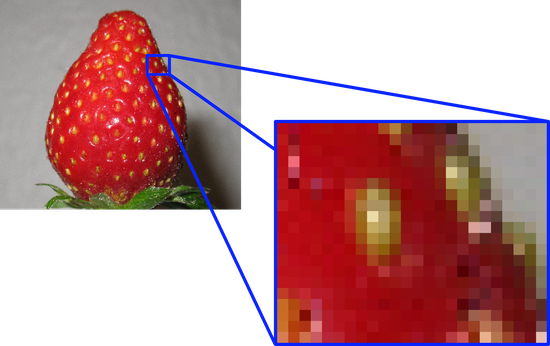
\includegraphics[trim=10 0 0 20,width=0.5\textwidth]{Images/codage_information/Zoom_sur_une_image}
	\caption{Une image préparée pour être affichée sur un écran est "découpée" en un tableau de pixels ayant chacun une couleur donnée.}
\end{figure}
Le codage d'image est un entreprise autrement plus complexe que le codage de texte. Commençons par une image en noir et blanc, dans ce cas chaque pixel est soit blanc, soit noir. Par conséquent le codage le plus simple est de représenter chaque pixel avec un 1 ou un 0. 

\begin{figure}[h!]
	\centering
	\subfloat{%
		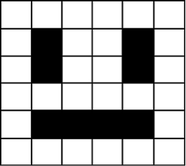
\includegraphics[trim=0 0 0 0,width=0.3\textwidth]{Images/codage_information/img_bin1}
	}
	\hspace{1cm}
	\subfloat{%
		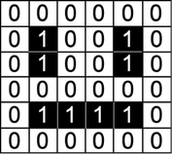
\includegraphics[trim=0 0 0 0,width=0.3\textwidth]{Images/codage_information/img_bin2}
	}
	\hspace{1cm}
	\subfloat{%
	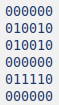
\includegraphics[trim=0 0 0 0,width=0.15\textwidth]{Images/codage_information/img_bin3}
	}
	\caption{Représentation d'une image binaire}
	\label{img_bin}
\end{figure}
Si on reprend l'exemple de la figure \ref{img_bin}, notre image pourrait être représentée par la suite de bits:\\
\hspace{1cm} 000000010010010010000000011110000000.\\
Cependant dans ce cas là, il faut aussi spécifier les dimensions de l'image pour que le codage soit complet (6 x 6 ici). On appelle ces données, les \textbf{méta-données}.
%\begin{mydefinition}
%	Les méta-données sont les données nécessaire à la reconstruction de l'
%\end{mydefinition}
	
\subsection{image en niveau de gris}
La vie est faite de nuance et les images en noir et blanc n'échappe pas à ce constat, il existe plusieurs nuances de gris entre le blanc et le noir. En général, ces niveaux de gris sont codés avec un octet ce qui permet 255 nuances entre le noir (codé avec nombre 0) et le blanc (codé avec le nombre $255=11111111_2$).

\begin{figure}[h!]
	\centering
	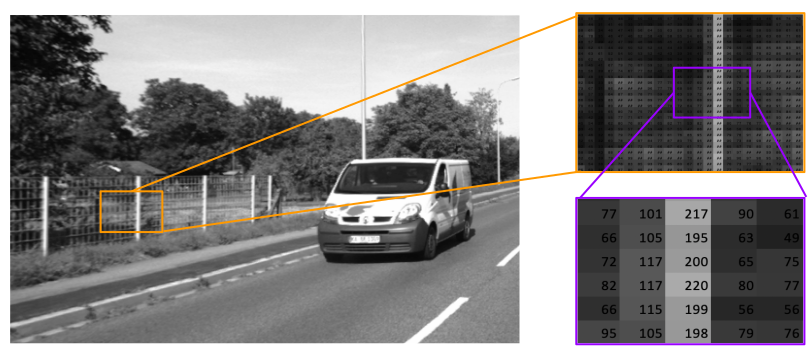
\includegraphics[trim=10 0 0 20,width=0.8\textwidth]{Images/codage_information/image_gris.png}
	\caption{Codage d'une image en niveau de gris. Chaque pixel est associé à un nombre entre 0 et 255 qui . Le nombres sur les pixels représentent l'intensité du niveau de gris, cette indication n'existe pas sur l'image d'origine (\textit{source: Informatique au gymnase}).}
\end{figure}

\subsection{Codage des couleurs*}
Les pixels de la plupart des écrans d'ordinateur sont composés de 3 "lampes" : une rouge, une verte et une bleue.

\begin{figure}[h!]
	\centering
	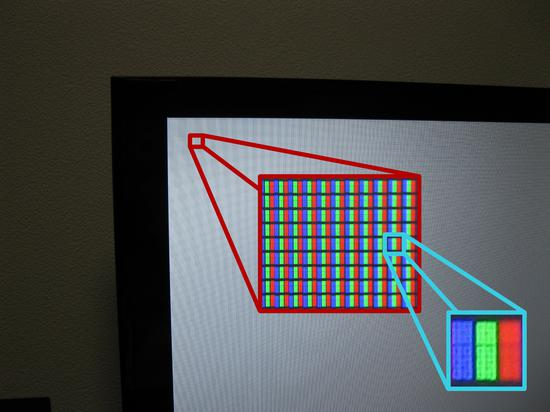
\includegraphics[trim=0 0 60 0,width=0.5\textwidth]{Images/codage_information/Zoom_sur_un_pixel.jpg}
	\caption{Zoom sur un pixel. On peut voir les pixels d'un écran en se rapprochant très près de celui-ci, ou avec une loupe (source: \textit{science-questions.org}).}
\end{figure}

\begin{wrapfigure}[]{r}{0.3\textwidth}
	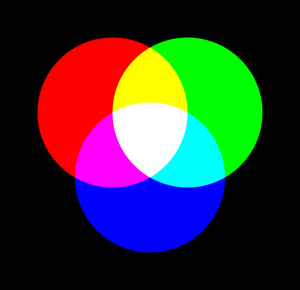
\includegraphics[trim=0 0 0 20,width=0.28\textwidth]{Images/codage_information/Addition_des_couleurs.png}
\end{wrapfigure}

\textit{Les pixels utilisent ainsi des propriétés d'additivité des couleurs qui permettent, à partir de trois couleurs, de générer un arc-en-ciel de couleurs du rouge au violet. Pour déterminer quelle couleur est obtenue en fonction des lumières allumées, on peut s'aider du schéma ci-dessous qui représente la superposition de trois projecteurs, rouge, vert et bleu (source: science-questions.org):}

%\begin{figure}[h!]
%	\centering
%	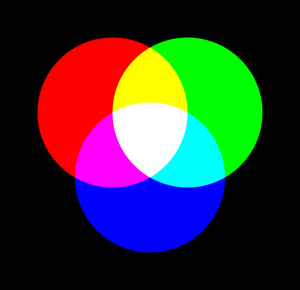
\includegraphics[trim=10 0 0 0,width=0.3\textwidth]{Images/codage_information/Addition_des_couleurs.png}
%	\caption{Addition des couleurs}
%\end{figure}
Pour le codage des images couleurs, on codera chaque pixel en utilisant 3 octets, ce qui donne
\begin{itemize}
	\item R: 255 nuance de rouge,
	\item G: 255 nuance de vert,
	\item B: 255 nuance de bleu.
\end{itemize}

\begin{figure}[h!]
	\centering
	\subfloat[Image originale]{%
		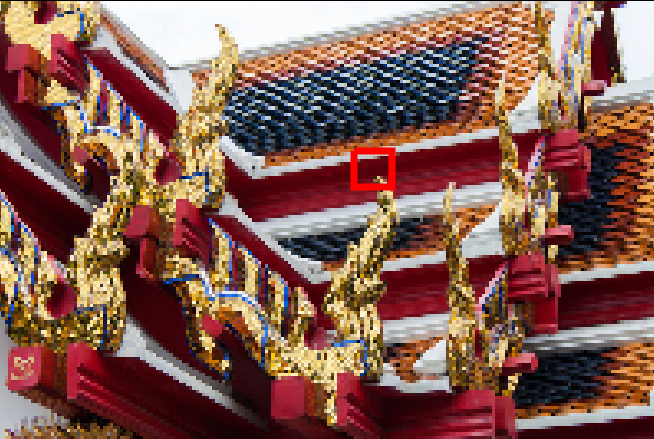
\includegraphics[trim=0 0 0 0,width=0.5\textwidth]{Images/codage_information/image_couleur}
	}
	\hspace{1cm}
	\subfloat[Zoom sur des pixels avec leurs valeurs RGB]{%
		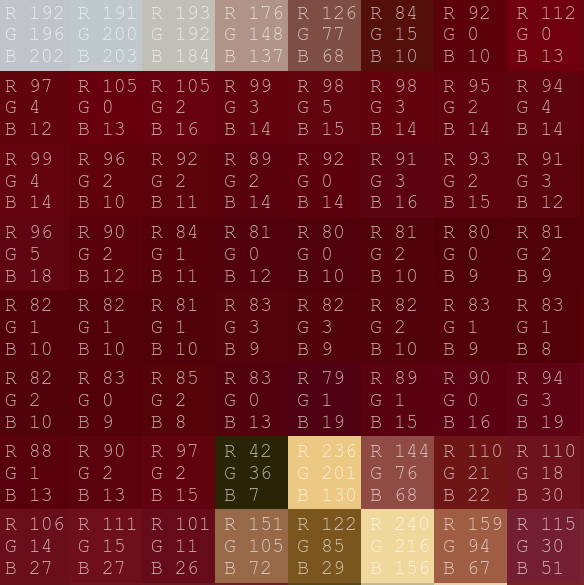
\includegraphics[trim=0 0 0 0,width=0.33\textwidth]{Images/codage_information/image_couleur_zoom}
	}
	\caption{chaque pixel d'une image est représenté avec 3 intensités de rouge(R), vert(G) et bleu(B) allant de 0 à 255 (codé chacune avec 1 octet).}
	\label{img_coul}
\end{figure}


\section{*Sons}
Sans empiéter dur le cours de physique, les sons peuvent être modélisés comme des signaux variant au cours du temps. Ces signaux sont converties sous forme des nombres à travers un processus comme appelle échantillonnage qui va déterminer les temps auquel on mesure le signaux et les différents niveaux d'intensité que sont possibles (ces niveaux sont codés en binaire).

\begin{figure}[h!]
	\centering
	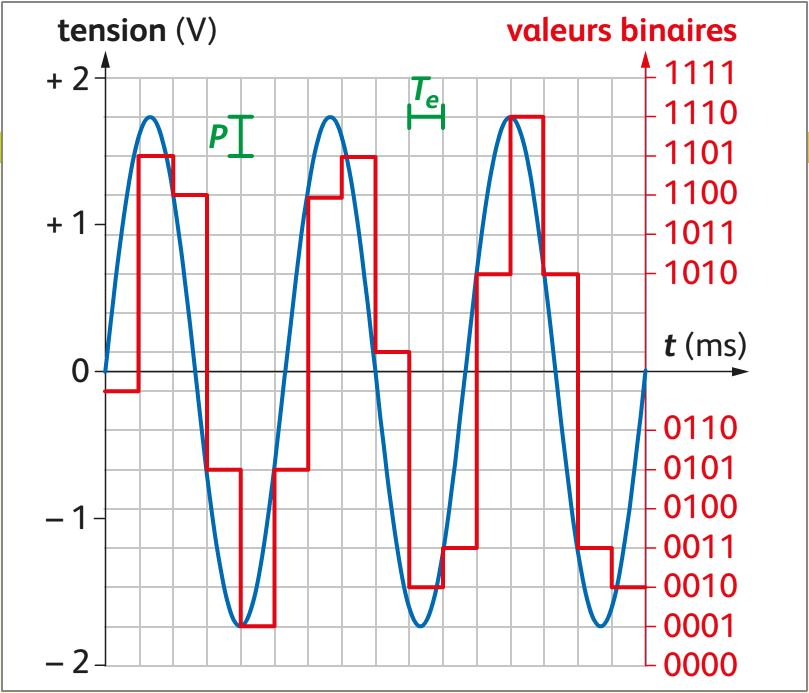
\includegraphics[trim=10 0 60 0,width=0.5\textwidth]{Images/codage_information/illustration_echantillonage.jpg}
	\caption{Exemple de numérisation d'un signal.}
\end{figure}
\vspace{-0.5cm}
\section{*Vidéos}
Les vidéos peuvent être représentées comme une succession d'image (par exemple, autour de 24  images par secondes afin que l’œil ne puisse pas distinguer les images qui défilent) associé avec du son. 